\begin{figure}[htp]
	\centering
	\subfloat[\(\mesh{\Phi}\)]
	{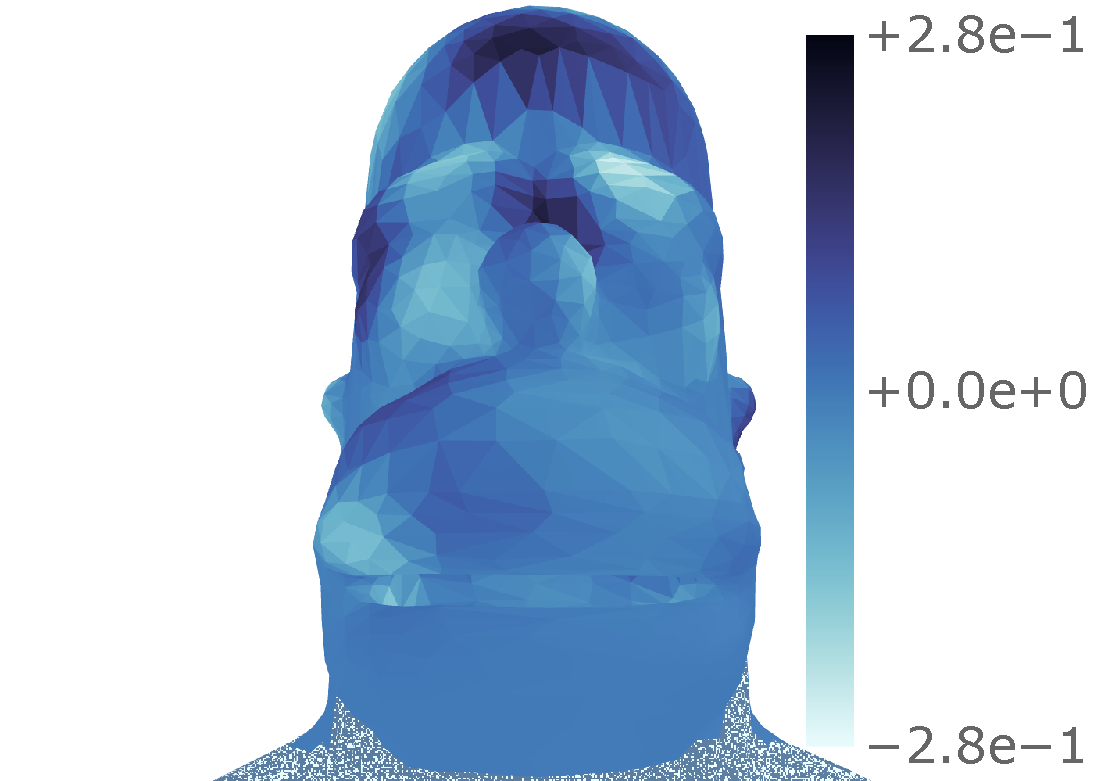
\includegraphics[trim={101 0 3 3},clip,width=.33\textwidth]{slepian_wavelets_homer_3B_2jmin_scaling_zoom.pdf}}
	\hfill
	\subfloat[\(\mesh{\Psi^{2j}}\)]
	{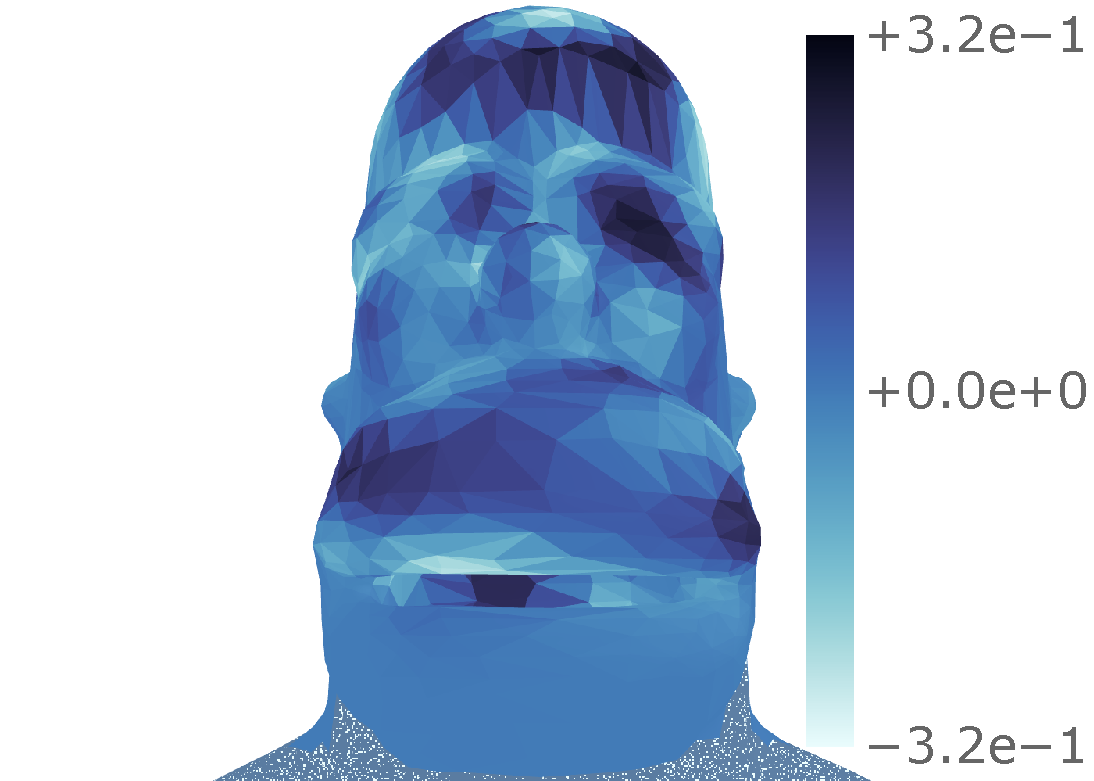
\includegraphics[trim={101 0 3 3},clip,width=.33\textwidth]{slepian_wavelets_homer_3B_2jmin_2j_zoom.pdf}}
	\hfill
	\subfloat[\(\mesh{\Psi^{3j}}\)]
	{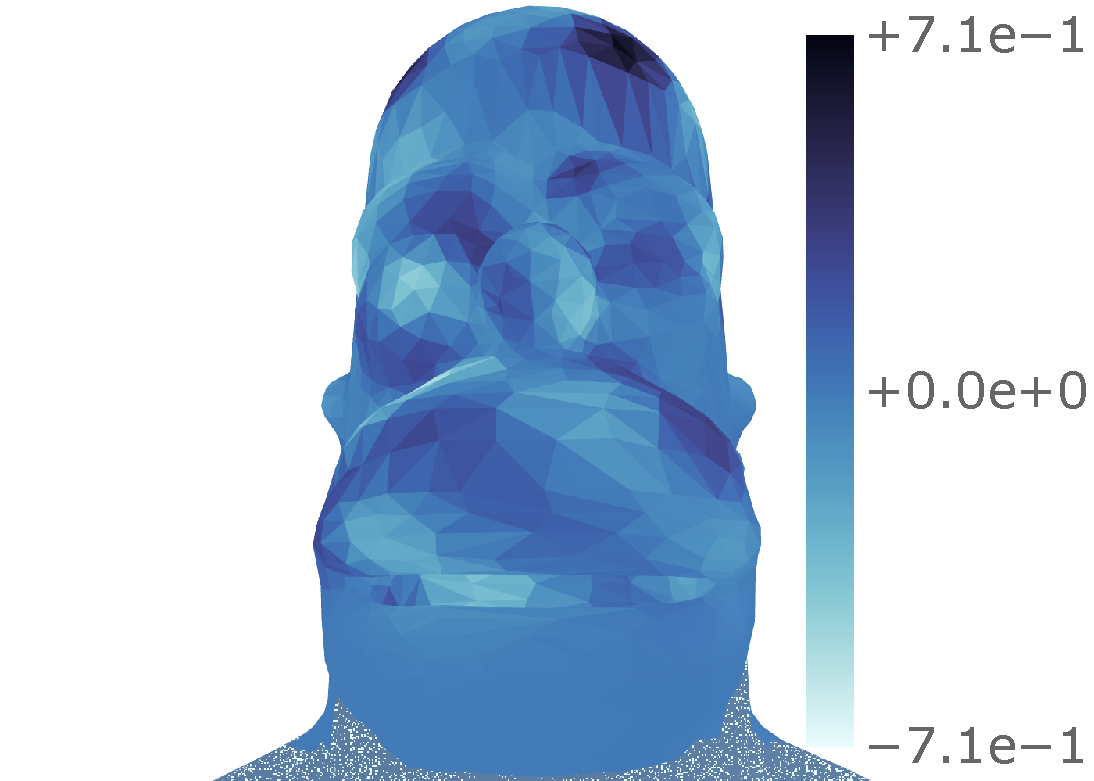
\includegraphics[trim={101 0 3 3},clip,width=.33\textwidth]{slepian_wavelets_homer_3B_2jmin_3j_zoom.pdf}}
	\newline
	\subfloat[\(\mesh{\Psi^{4j}}\)]
	{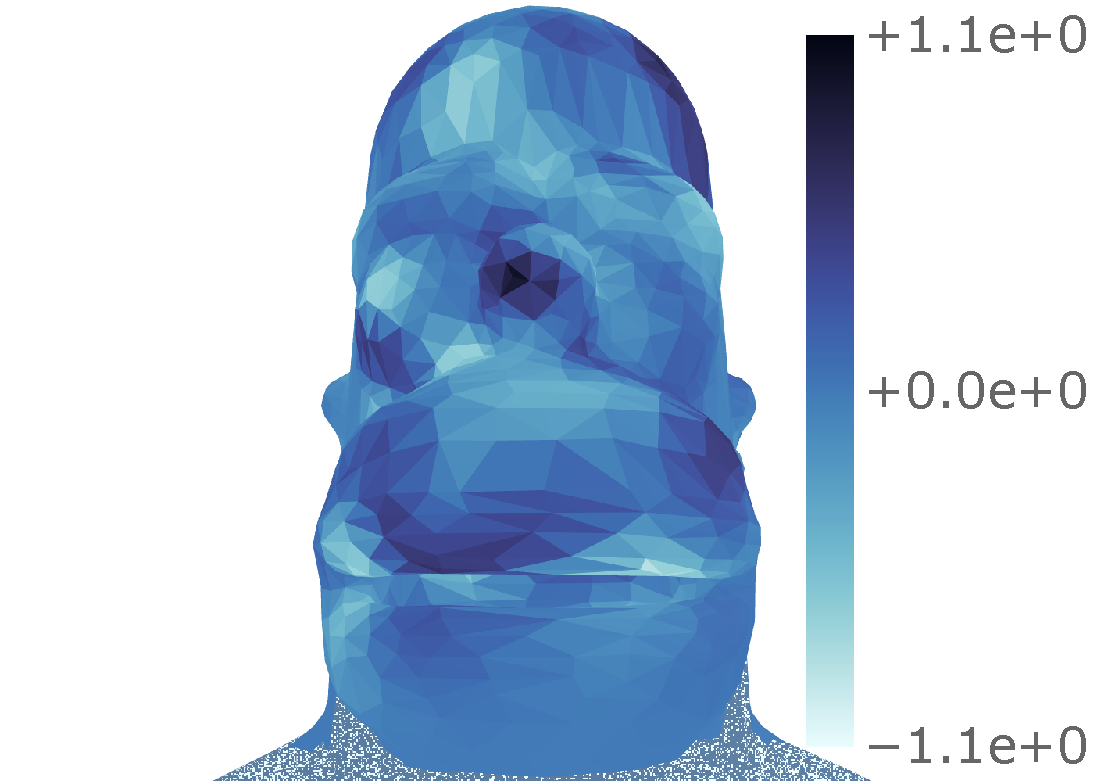
\includegraphics[trim={101 0 3 3},clip,width=.33\textwidth]{slepian_wavelets_homer_3B_2jmin_4j_zoom.pdf}}
	\hfill
	\subfloat[\(\mesh{\Psi^{5j}}\)]
	{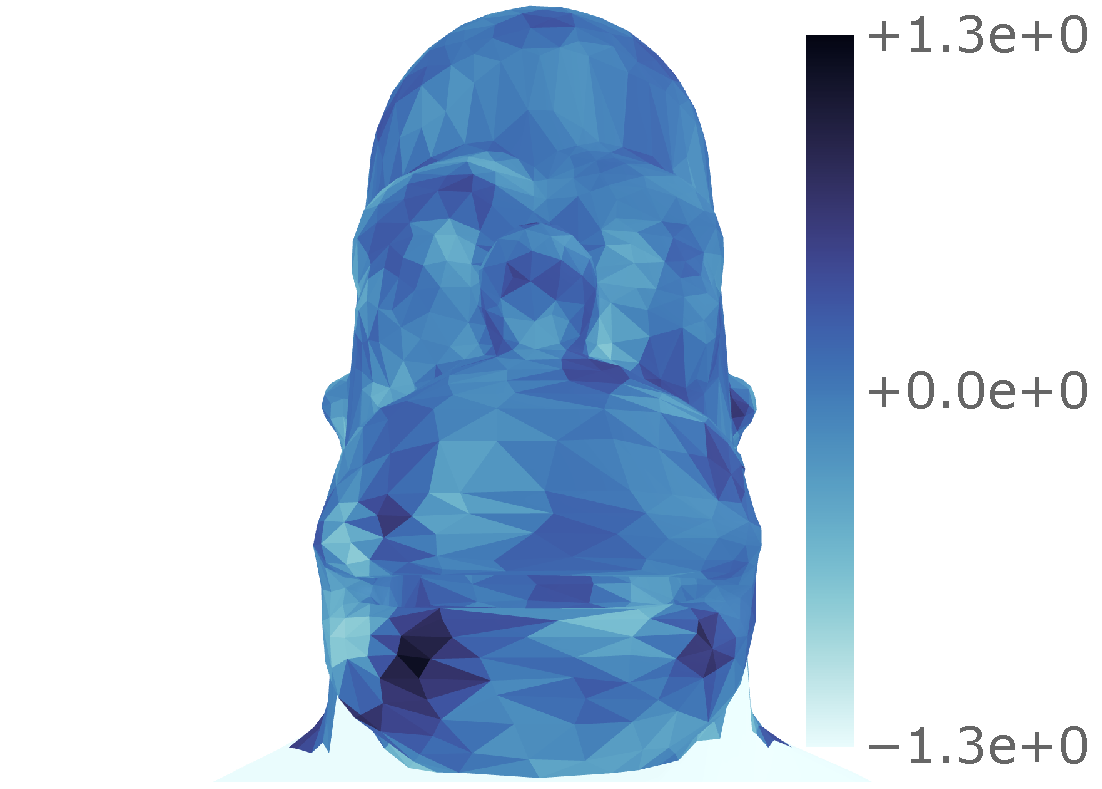
\includegraphics[trim={101 0 3 3},clip,width=.33\textwidth]{slepian_wavelets_homer_3B_2jmin_5j_zoom.pdf}}
	\hfill
	\subfloat[\(\mesh{\Psi^{6j}}\)]
	{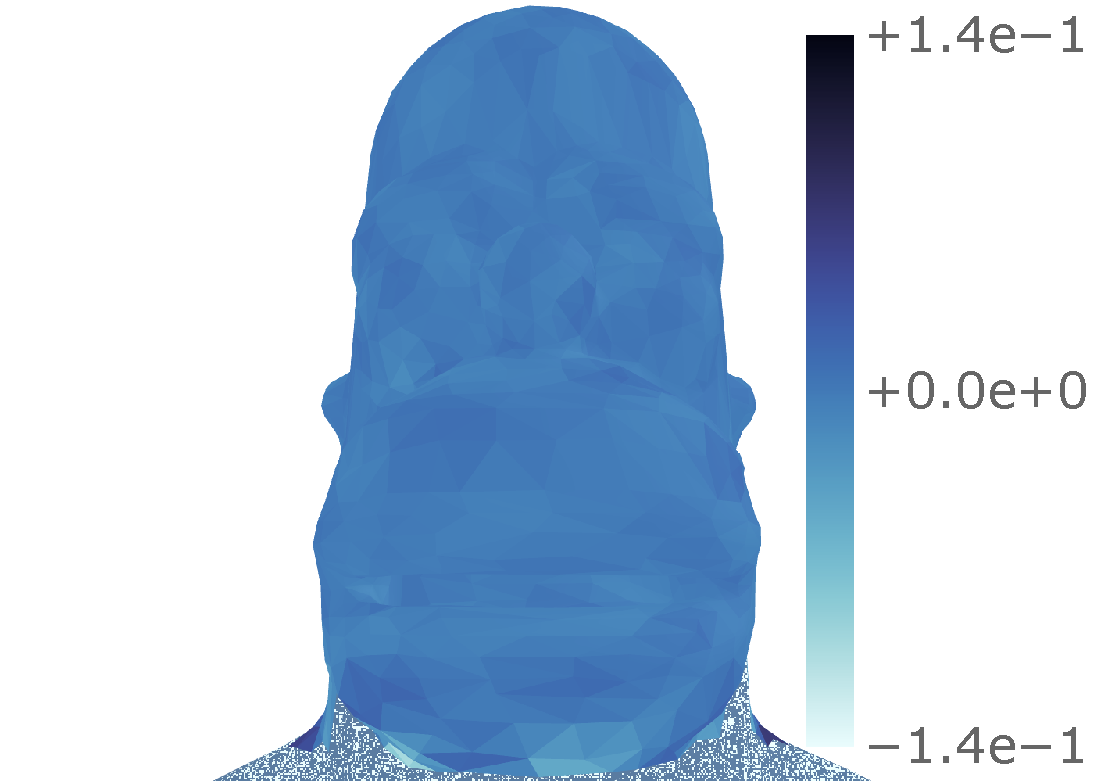
\includegraphics[trim={101 0 3 3},clip,width=.33\textwidth]{slepian_wavelets_homer_3B_2jmin_6j_zoom.pdf}}
	\caption{
	}\label{fig:chapter4_wavelets}
\end{figure}
